\documentclass[12pt]{article}

\usepackage[utf8]{inputenc}
\usepackage[spanish]{babel}
\usepackage{amsmath}
\usepackage{graphicx}
\usepackage{float}
\usepackage{booktabs}
\usepackage[a4paper, margin=2.5cm]{geometry}

\title{Análisis Estadístico de Chile utilizando datos reales de OECD}
\author{MIA CITLALI HERNANDEZ RODRIGUEZ}
\date{\today}

\begin{document}

\maketitle

\tableofcontents

\newpage

% =========================================================
% INTRODUCCIÓN
% =========================================================

\section{Introducción}

El presente trabajo muestra un análisis estadístico utilizando datos reales de Chile obtenidos mediante la API oficial de OECD. Los datos representan el comercio total del país entre los años 2015 y 2024.

A partir de estos datos se realizaron diferentes procedimientos estadísticos como medidas de tendencia central, medidas de dispersión, probabilidad, distribuciones estadísticas e índices económicos. Además, se generaron gráficas en Python para visualizar mejor el comportamiento comercial de Chile.

La información utilizada fue obtenida mediante la API oficial de OECD:

\begin{verbatim}
https://sdmx.oecd.org/sti-public/rest/data/
OECD.STI.PIE,DSD_BTIGE@DF_BTIGE,1.0/
A.CHL.X.TOTAL..W.
\end{verbatim}

Los cálculos y gráficas fueron realizados en Python utilizando Google Colab y posteriormente documentados en \LaTeX.

% =========================================================
% CANTIDAD TOTAL DE DATOS
% =========================================================

\section{Cantidad Total de Datos}

\subsection*{Problema}

Determinar cuántos registros fueron utilizados para el análisis estadístico de Chile.

\subsection*{Resultado}

\[10\]

\subsection*{Interpretación}

Se trabajó con 10 registros correspondientes al comercio total de Chile entre 2015 y 2024, permitiendo realizar comparaciones estadísticas y análisis de crecimiento económico.

% =========================================================
% DATOS UTILIZADOS
% =========================================================

\section{Datos utilizados}

\begin{table}[H]
\centering
\begin{tabular}{cc}
\toprule
Año & Comercio Total \\
\midrule
2015 & 341722204.203 \\
2016 & 332096808.103 \\
2017 & 379820506.797 \\
2018 & 410813086.393 \\
2019 & 376021711.371 \\
2020 & 410892923.035 \\
2021 & 530867045.654 \\
2022 & 540771761.392 \\
2023 & 522857743.933 \\
2024 & 548051873.416 \\
\bottomrule
\end{tabular}
\caption{Datos comerciales de Chile obtenidos de OECD}
\end{table}

% =========================================================
% GRAFICA GENERAL
% =========================================================

\section{Gráfica general del comercio}

\begin{figure}[H]
\centering
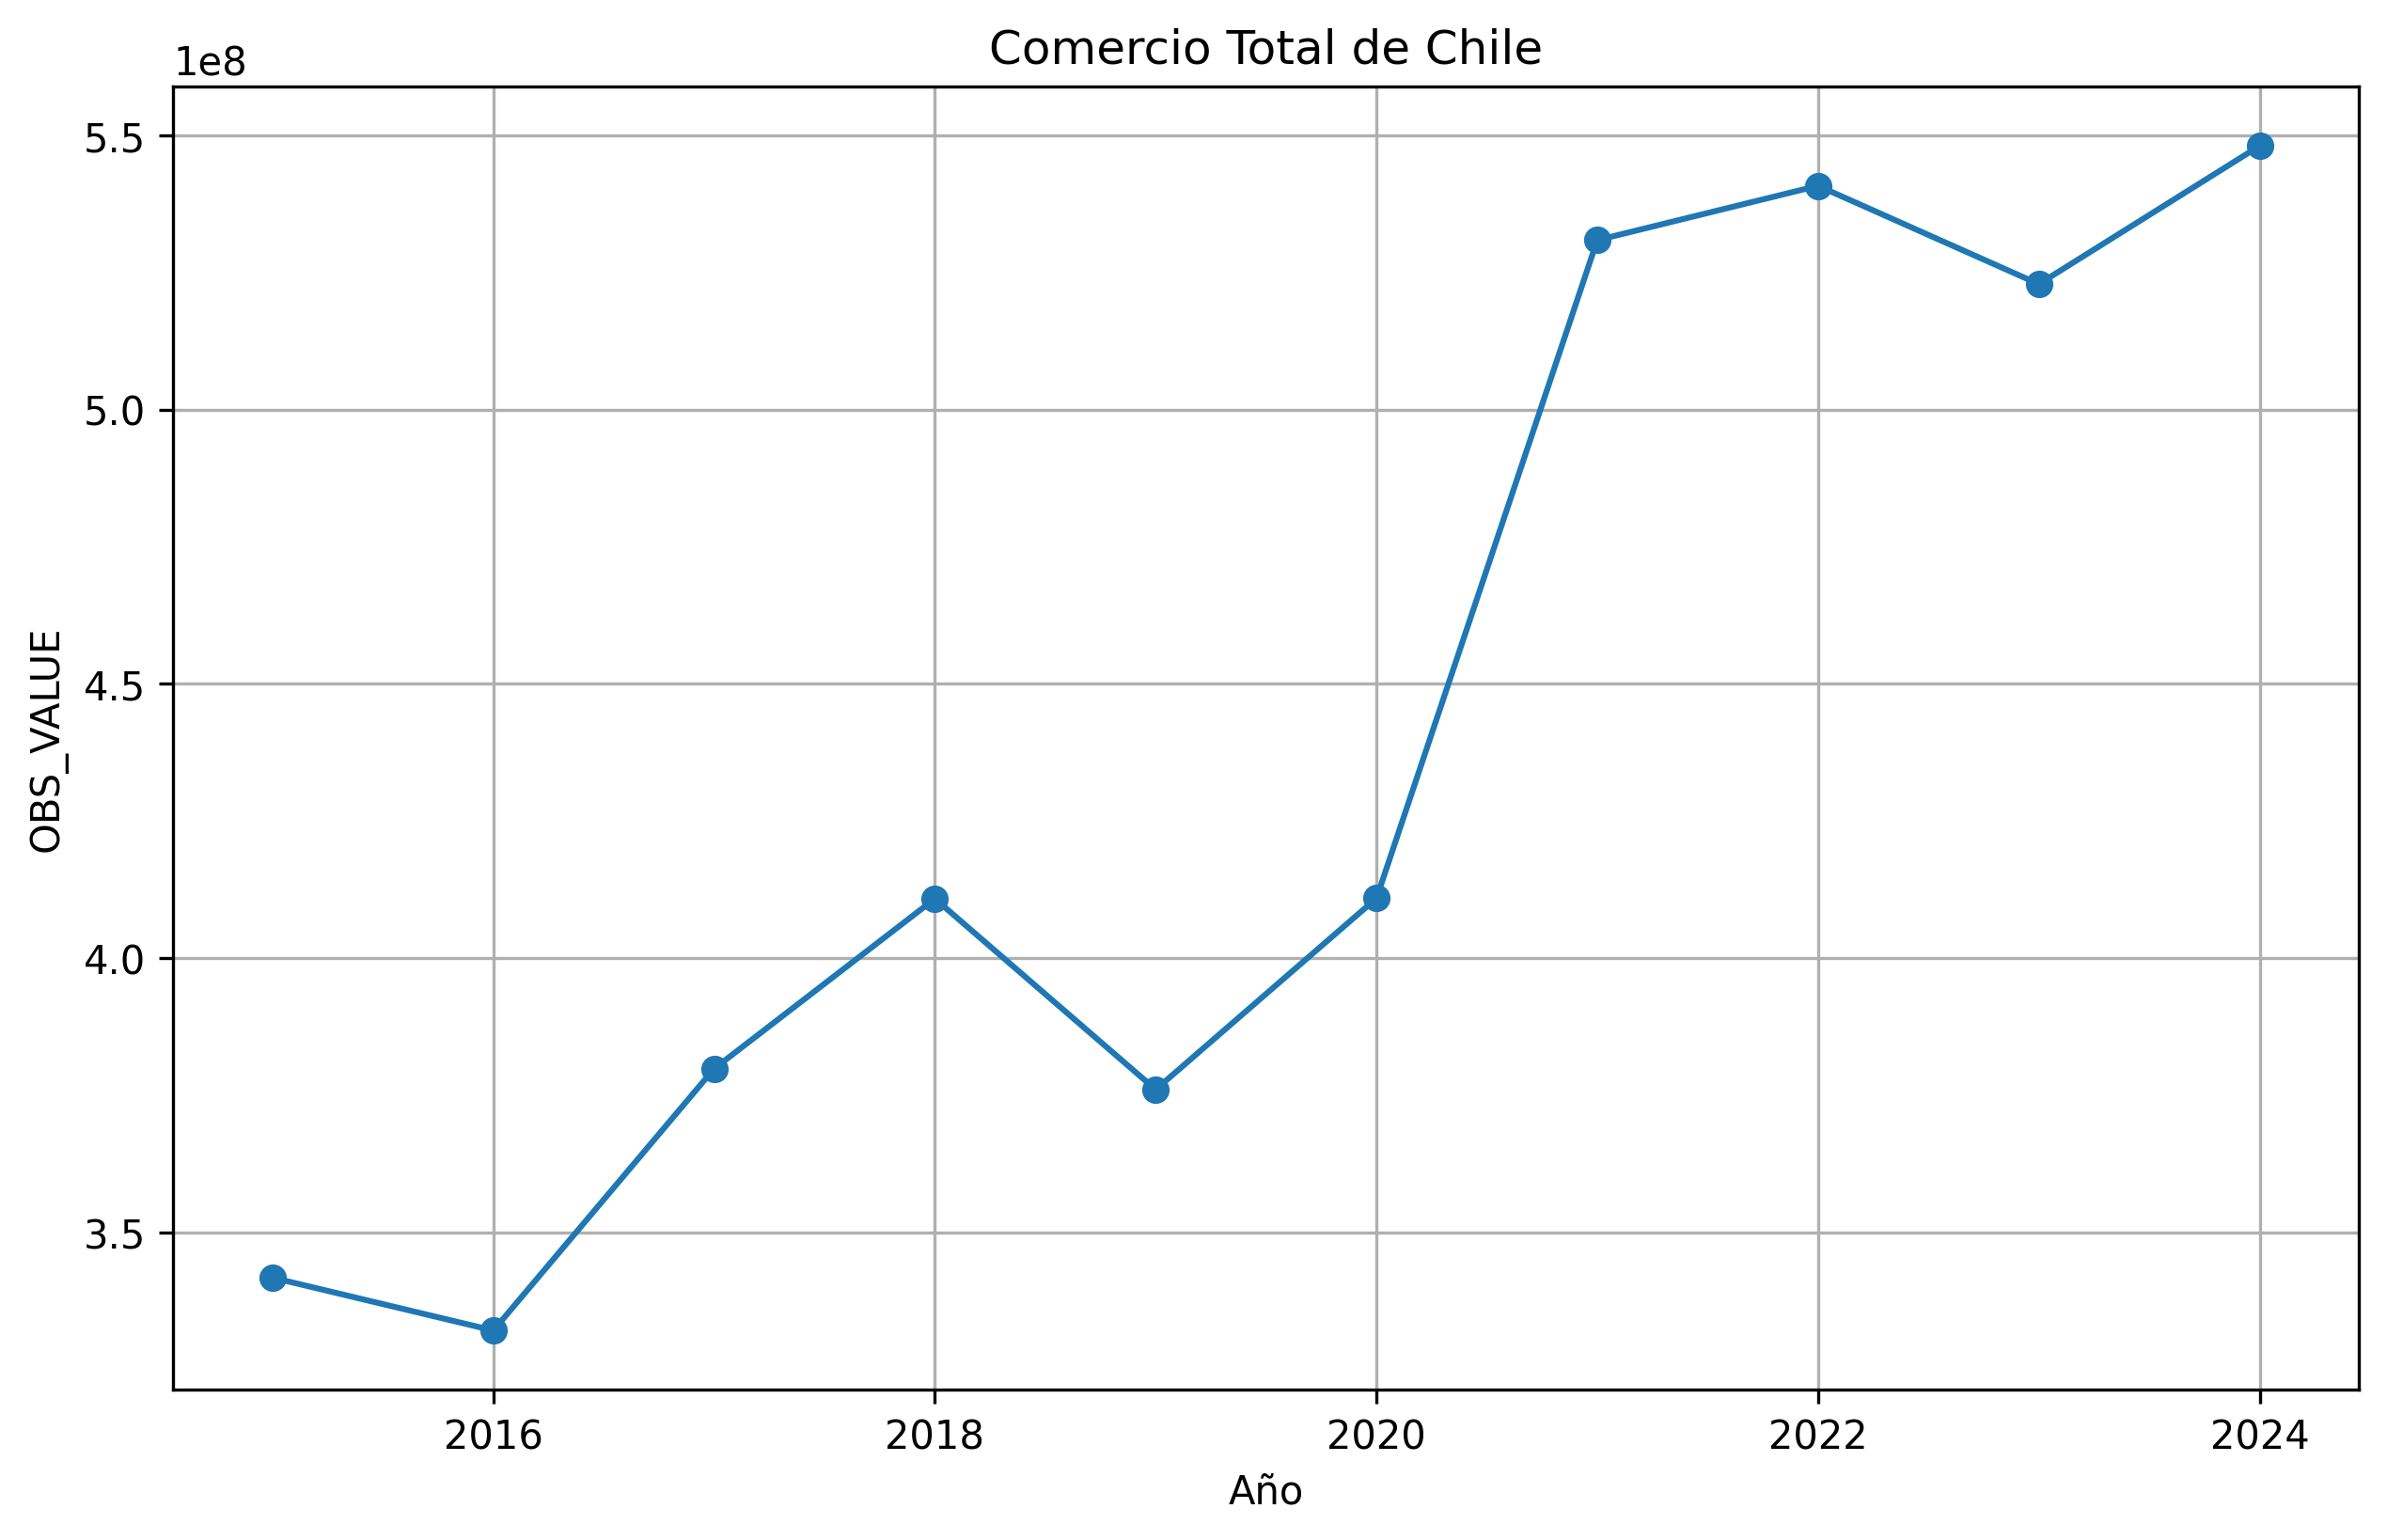
\includegraphics[width=0.9\textwidth]{grafica1.png}
\caption{Comercio total de Chile}
\end{figure}

\textbf{Interpretación de la gráfica}

La gráfica muestra que el comercio chileno presentó un crecimiento importante principalmente después del año 2020. Los años 2021, 2022 y 2024 registraron algunos de los valores más altos del periodo analizado.

% =========================================================
% DATOS AGRUPADOS
% =========================================================

\section{Datos Agrupados}

\subsection{Moda Agrupada}

\subsection*{Problema}

Identificar el intervalo con mayor frecuencia dentro de los datos agrupados del comercio chileno.

\subsection*{Resultado}

\[
(331880853.038,\ 386085574.431]
\]

\subsection*{Interpretación}

La mayor concentración de datos comerciales de Chile se encuentra dentro de este intervalo.

% =========================================================

\subsection{Mediana Agrupada}

\subsection*{Problema}

Encontrar el valor central de los datos agrupados.

\subsection*{Resultado}

\[
410853004.714
\]

\subsection*{Interpretación}

La mitad de los valores comerciales de Chile se encuentran por debajo de este valor y la otra mitad por encima.

% =========================================================

\subsection{Media Agrupada}

\subsection*{Problema}

Calcular el promedio de los datos agrupados del comercio chileno.

\subsection*{Resultado}

\[
439391566.4297
\]

\subsection*{Interpretación}

La media agrupada representa el comportamiento promedio del comercio de Chile durante el periodo estudiado.

% =========================================================
% MODA
% =========================================================

\section{Medidas de Tendencia Central}

\subsection{Moda}

\subsection*{Problema}

Encontrar el valor comercial que más se repite.

\subsection*{Fórmula}

\[
Mo = \text{valor que más se repite}
\]

\subsection*{Resultado}

\[
Mo = 332096808.103
\]

\subsection*{Interpretación}

Uno de los valores comerciales más frecuentes de Chile fue aproximadamente 332 millones.

% =========================================================
% MEDIANA
% =========================================================

\subsection{Mediana}

\subsection*{Problema}

Calcular el valor central del comercio chileno.

\subsection*{Fórmula}

\[
Md = \frac{x_{n/2}+x_{(n/2)+1}}{2}
\]

\subsection*{Sustitución}

\[
Md = \frac{410813086.393 + 410892923.035}{2}
\]

\subsection*{Resultado}

\[
Md = 410853004.714
\]

\subsection*{Interpretación}

La mitad de los años tuvieron valores menores a 410 millones y la otra mitad mayores.

% =========================================================
% MEDIA
% =========================================================

\subsection{Media}

\subsection*{Problema}

Calcular el promedio del comercio total de Chile.

\subsection*{Fórmula}

\[
\bar{x}=\frac{\sum x_i}{n}
\]

\subsection*{Sustitución}

\[
\bar{x}=\frac{4393915664.297}{10}
\]

\subsection*{Resultado}

\[
\bar{x}=439391566.4297
\]

\subsection*{Interpretación}

El comercio promedio anual de Chile fue aproximadamente de 439 millones.

% =========================================================
% GRAFICA MEDIA
% =========================================================

\begin{figure}[H]
\centering
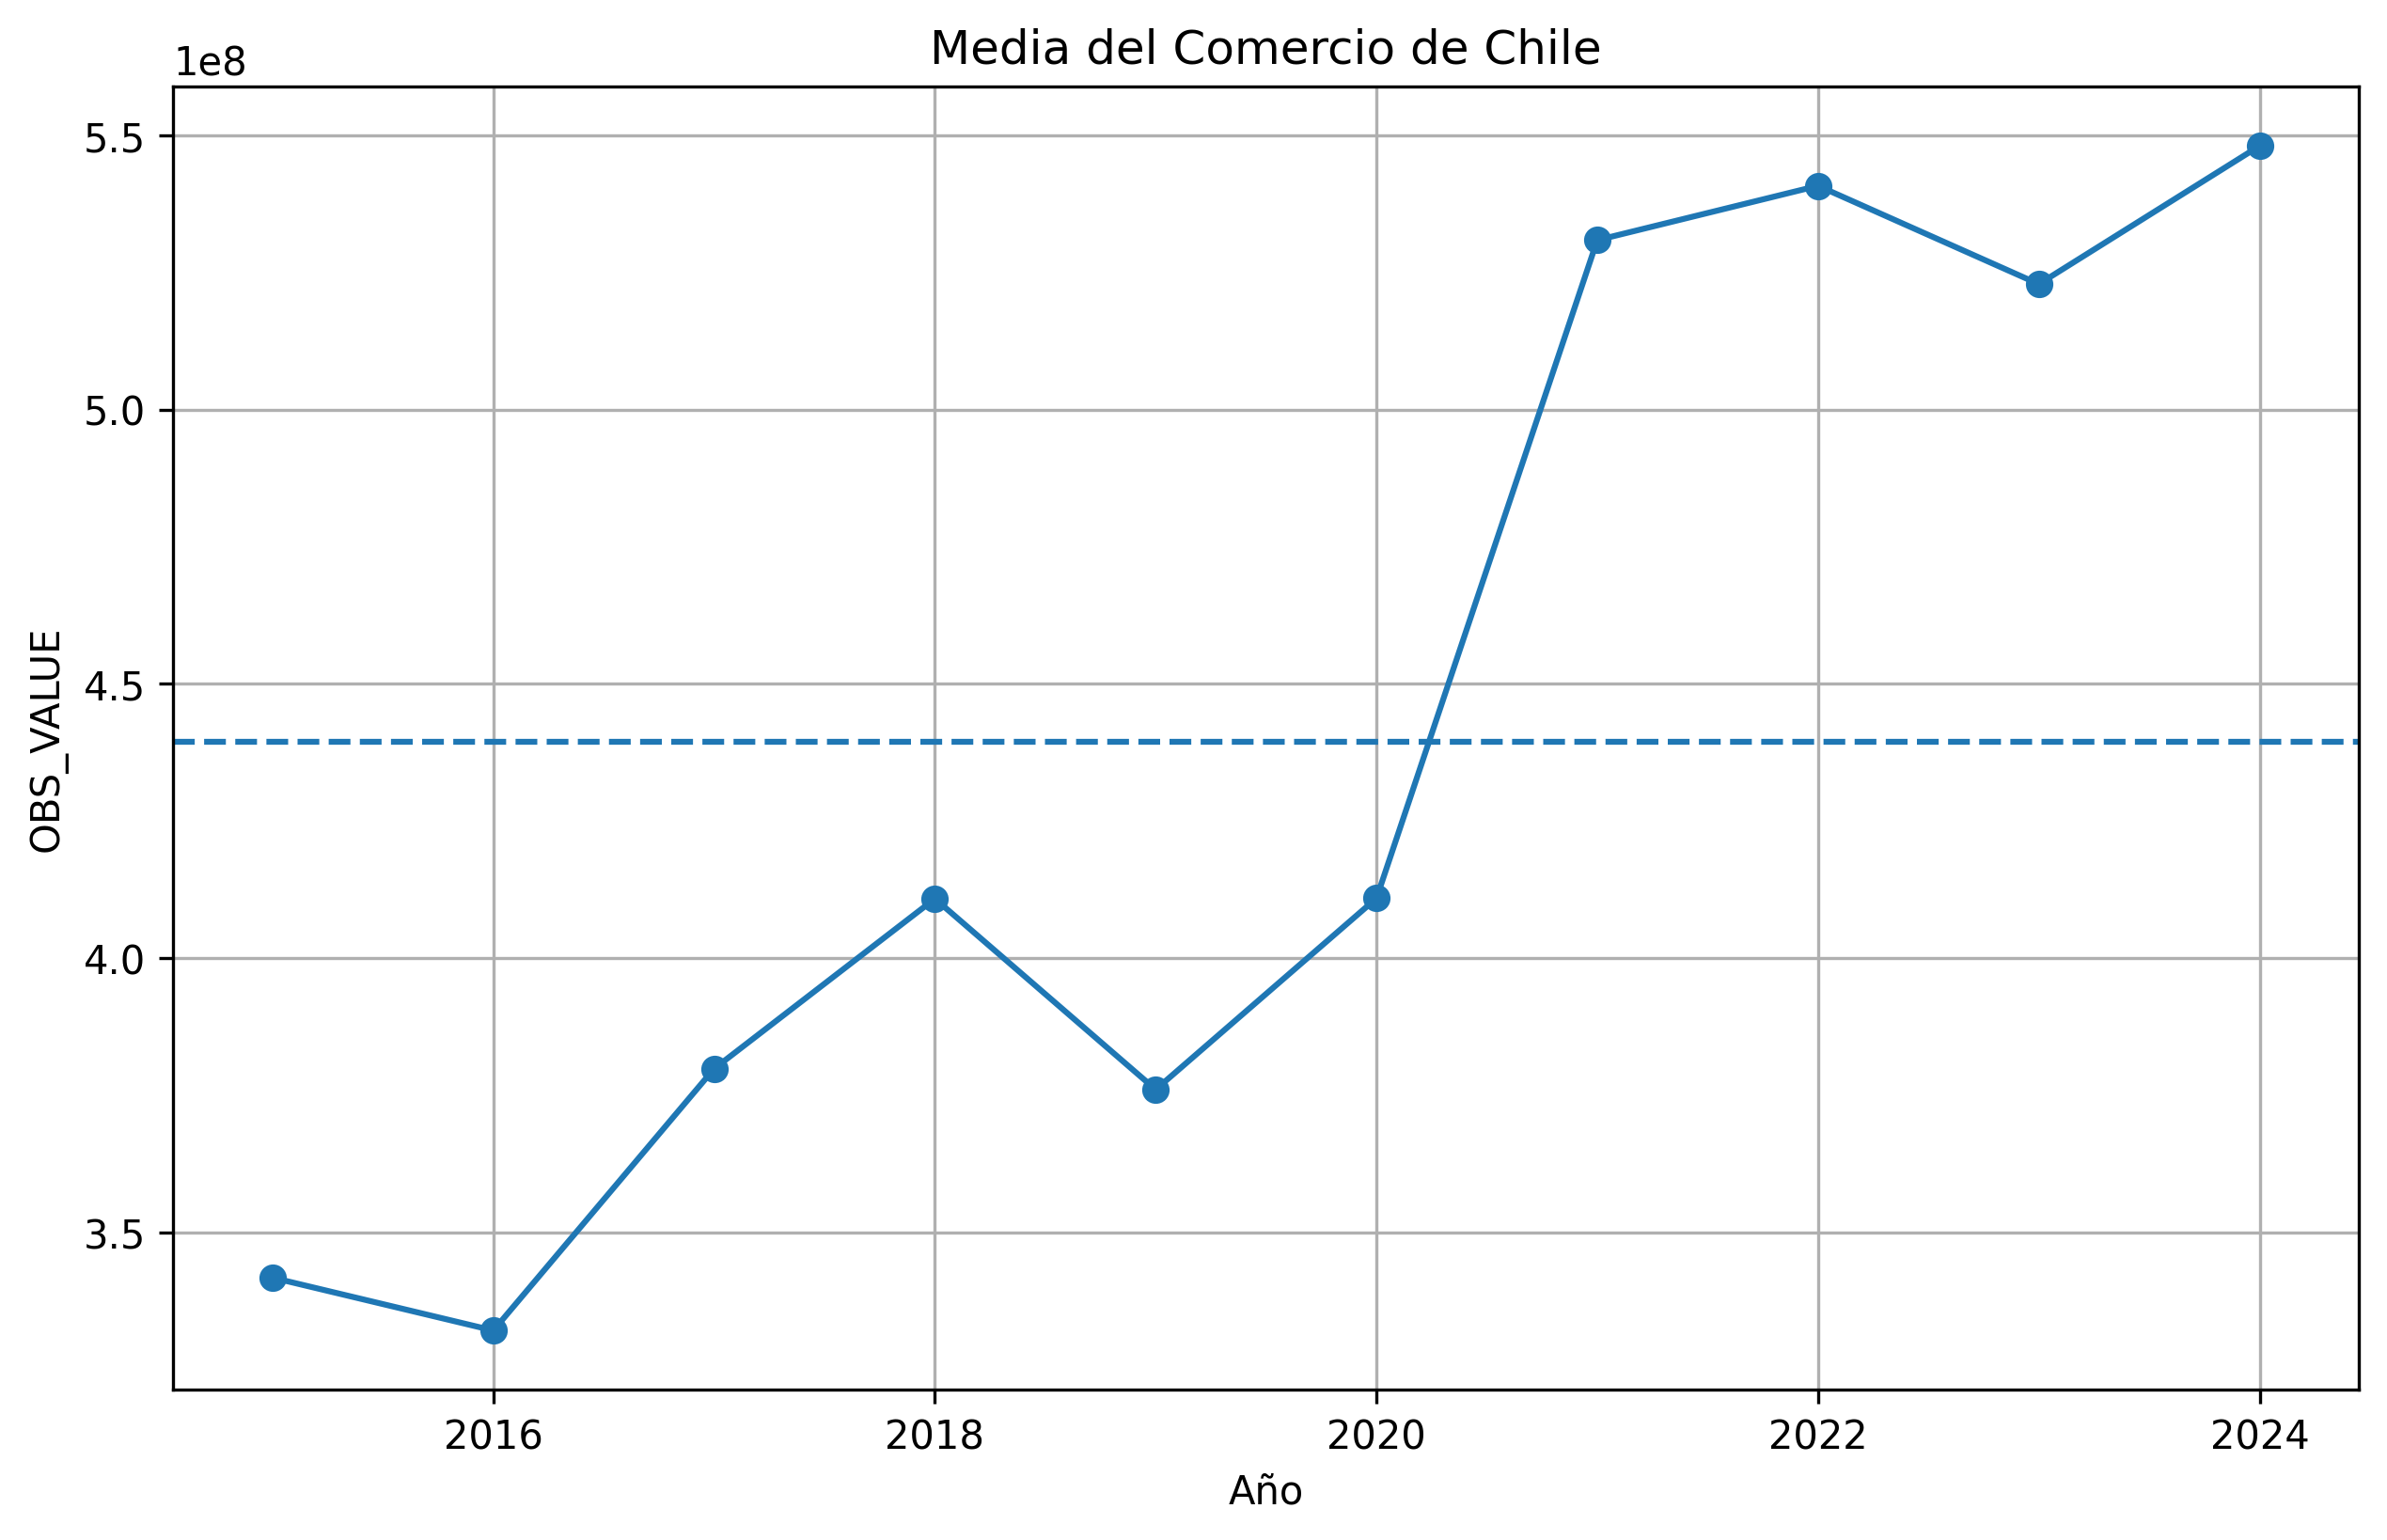
\includegraphics[width=0.9\textwidth]{grafica2.png}
\caption{Media del comercio de Chile}
\end{figure}

\textbf{Interpretación de la gráfica}

La línea de la media permite observar qué años estuvieron por encima y cuáles estuvieron por debajo del promedio general del comercio chileno.

% =========================================================
% DISPERSION
% =========================================================

\section{Medidas de Dispersión}

% =========================================================
% RANGO
% =========================================================

\subsection{Rango}

\subsection*{Problema}

Calcular la diferencia entre el mayor y menor valor del comercio chileno.

\subsection*{Fórmula}

\[
R = x_{max} - x_{min}
\]

\subsection*{Sustitución}

\[
R = 548051873.416 - 332096808.103
\]

\subsection*{Resultado}

\[
R = 215955065.313
\]

\subsection*{Interpretación}

Existe una diferencia importante entre los años de menor y mayor comercio de Chile.

% =========================================================
% RIQ
% =========================================================

\subsection{Rango Intercuartílico}

\subsection*{Problema}

Calcular el intervalo donde se concentra la mayor parte de los datos.

\subsection*{¿Por qué 25/100 y 75/100?}

El valor 25/100 representa el primer cuartil (Q1) y 75/100 representa el tercer cuartil (Q3).

\subsection*{Fórmula}

\[
RIQ = Q3 - Q1
\]

\subsection*{Sustitución}

\[
RIQ = 528864720.22375 - 376971410.22749
\]

\subsection*{Resultado}

\[
RIQ = 151893309.99625
\]

\subsection*{Interpretación}

La mayoría de los datos comerciales de Chile se encuentran dentro de este intervalo.

% =========================================================
% BOXPLOT
% =========================================================

\begin{figure}[H]
\centering
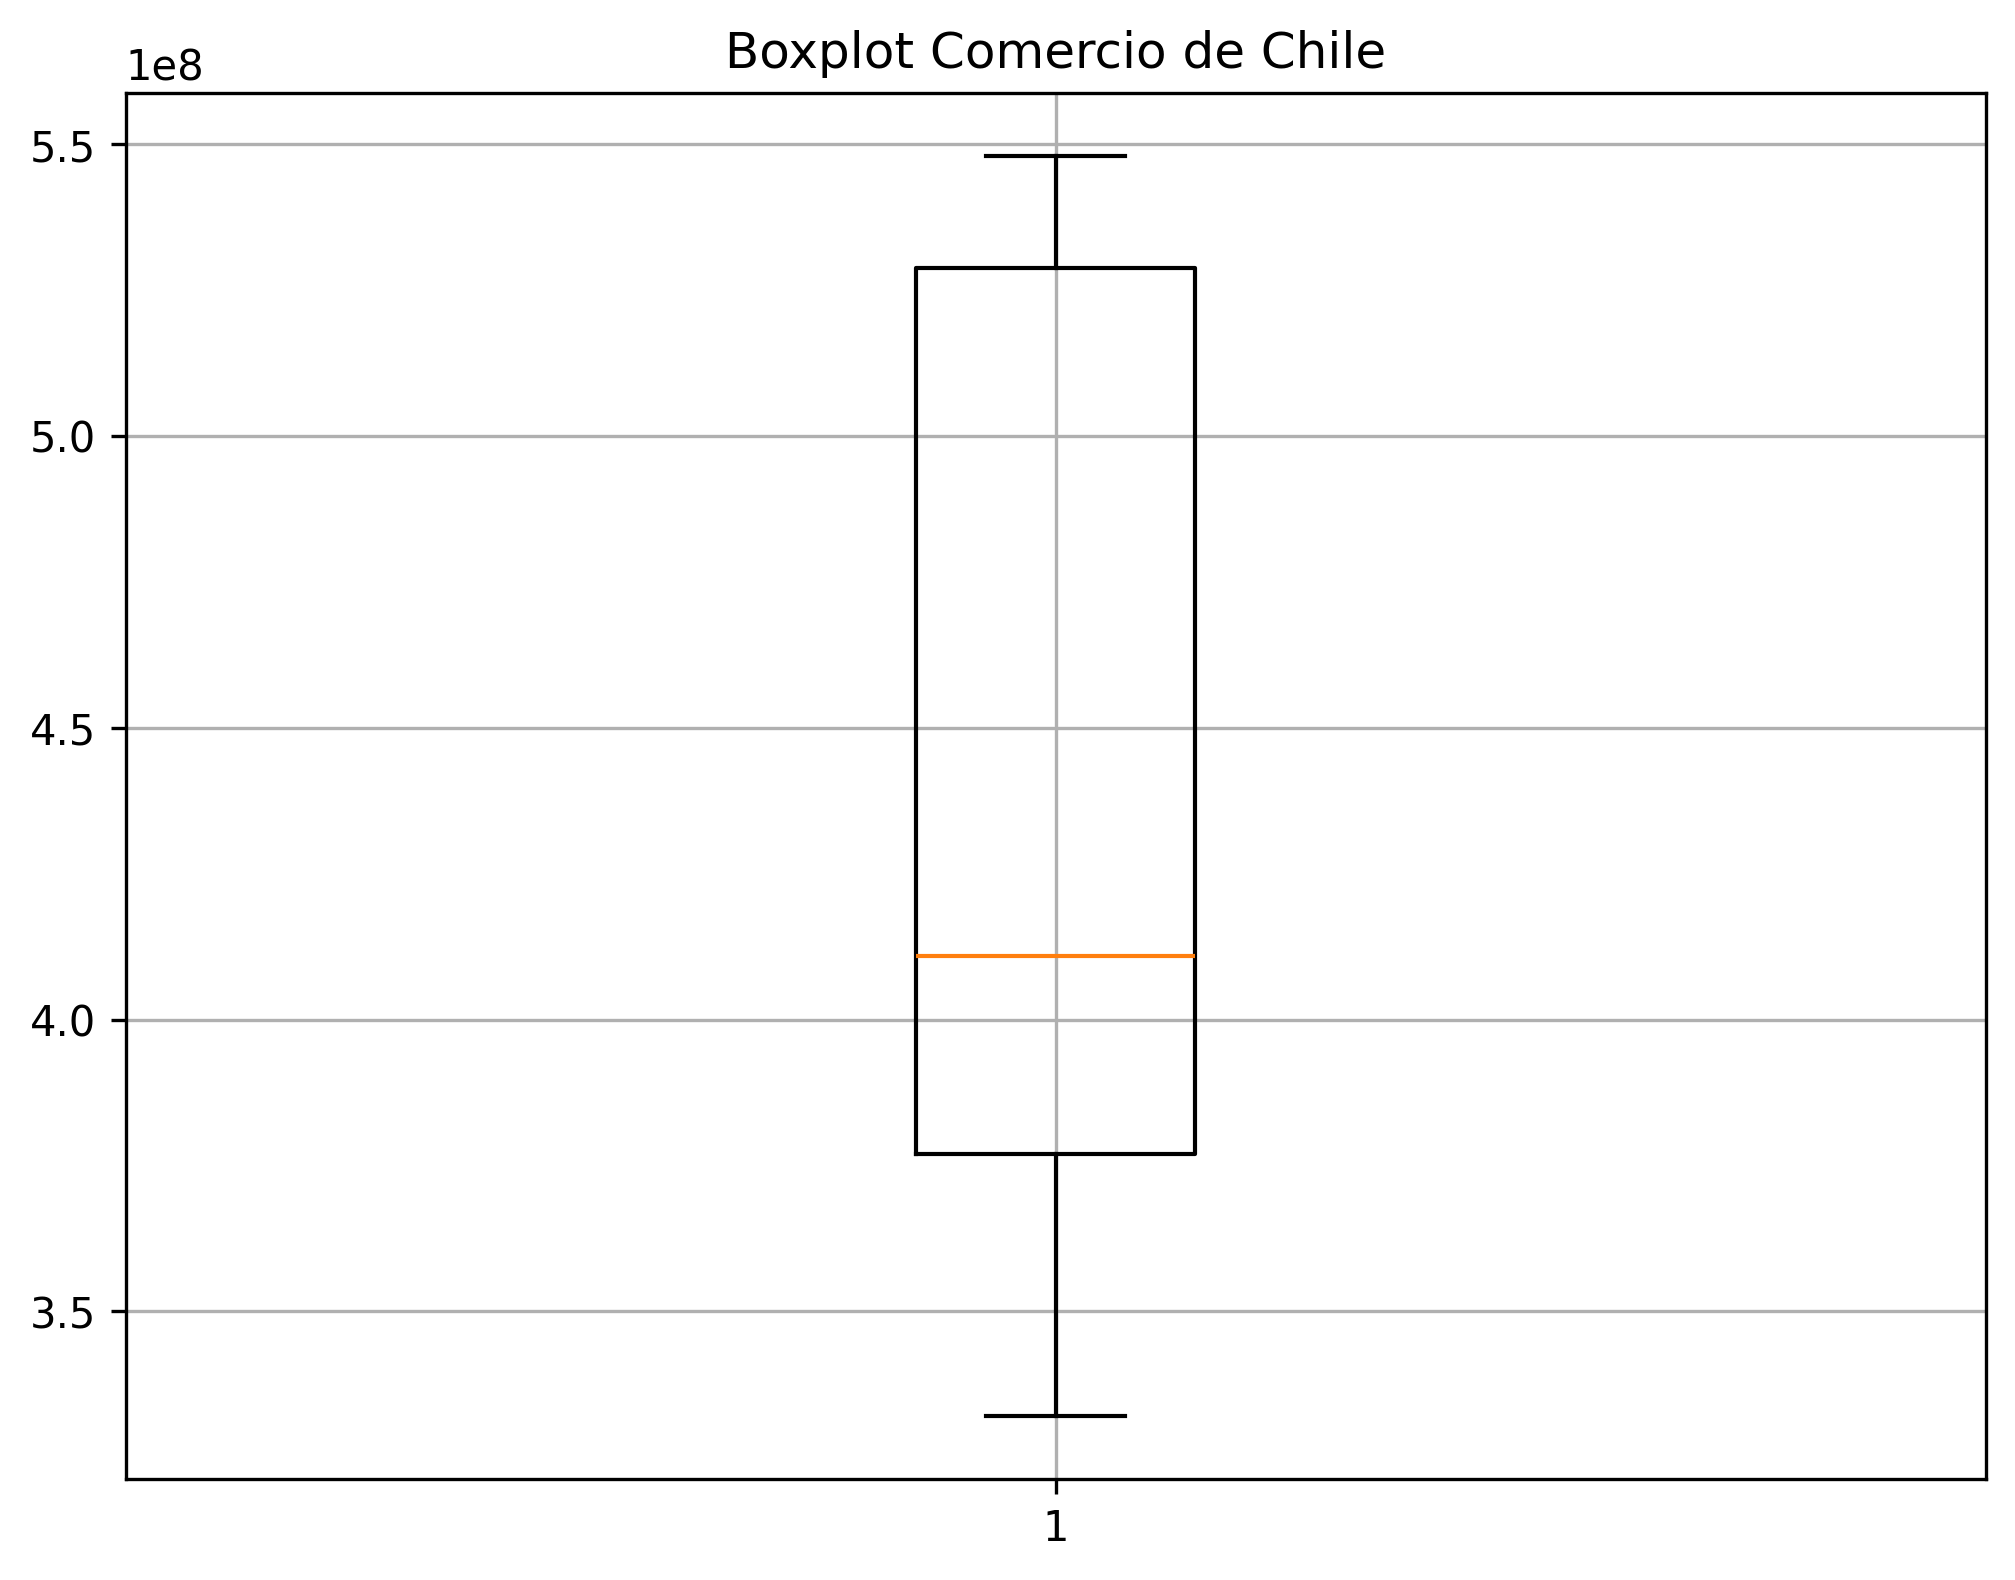
\includegraphics[width=0.7\textwidth]{grafica3.png}
\caption{Boxplot del comercio chileno}
\end{figure}

\textbf{Interpretación de la gráfica}

El boxplot permite observar la distribución de los datos comerciales de Chile, así como la dispersión y posibles valores extremos.

% =========================================================
% VARIANZA
% =========================================================

\subsection{Varianza}

\subsection*{Problema}

Medir la dispersión de los datos respecto a la media.

\subsection*{Fórmula}

\[
s^2 = \frac{\sum (x_i-\bar{x})^2}{n-1}
\]

\subsection*{Resultado}

\[
7518243742878177.0
\]

\subsection*{Interpretación}

Existe una variación importante en el comportamiento comercial de Chile durante el periodo estudiado.

% =========================================================
% DESVIACIÓN ESTÁNDAR
% =========================================================

\subsection{Desviación estándar}

\subsection*{Problema}

Calcular cuánto se alejan los datos respecto al promedio.

\subsection*{Fórmula}

\[
s = \sqrt{s^2}
\]

\subsection*{Resultado}

\[
86707806.7008858
\]

\subsection*{Interpretación}

Los datos se alejan aproximadamente 86 millones respecto a la media del comercio chileno.

% =========================================================
% DESVIACIÓN MEDIA
% =========================================================

\subsection{Desviación media}

\subsection*{Problema}

Calcular el alejamiento promedio absoluto.

\subsection*{Fórmula}

\[
DM = \frac{\sum |x_i-\bar{x}|}{n}
\]

\subsection*{Resultado}

\[
76996431.73524
\]

\subsection*{Interpretación}

El comercio chileno presenta una variación promedio considerable entre los distintos años analizados.

% =========================================================
% PROBABILIDAD
% =========================================================

\section{Probabilidad}

% =========================================================
% DIAGRAMA DE VENN
% =========================================================

\subsection{Diagrama de Venn}

\subsection*{Problema}

Comparar los años con crecimiento económico y los años con comercio superior a la media.

\subsection*{Conjunto A}

Años con crecimiento económico:

\[
\{2017,2018,2020,2021,2022,2024\}
\]

\subsection*{Conjunto B}

Años con comercio superior a la media:

\[
\{2021,2022,2023,2024\}
\]

\begin{figure}[H]
\centering
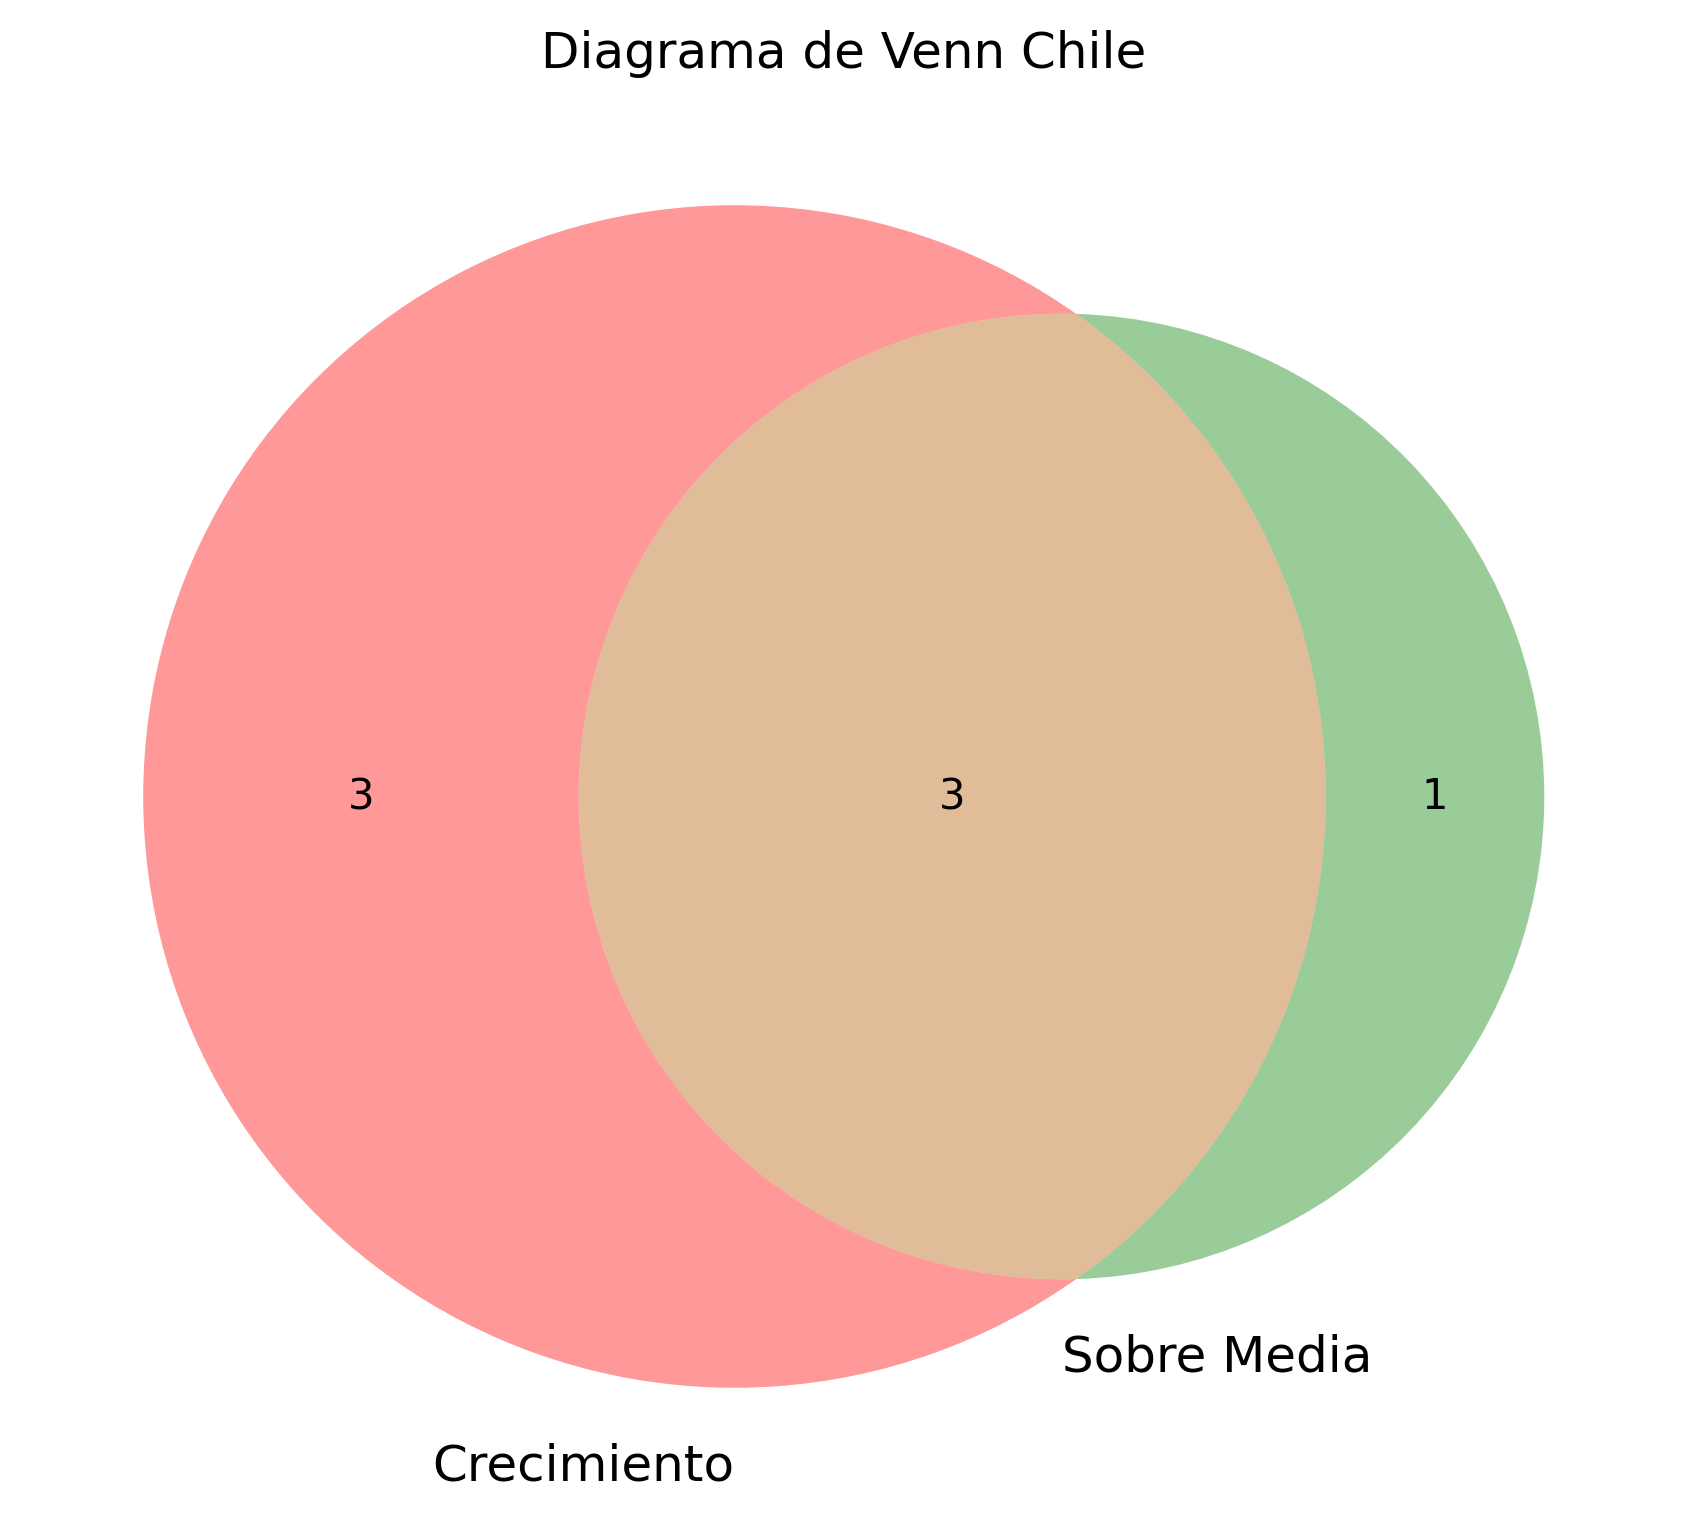
\includegraphics[width=0.7\textwidth]{grafica4.png}
\caption{Diagrama de Venn}
\end{figure}

\subsection*{Interpretación}

La intersección representa los años donde Chile tuvo crecimiento económico y además el comercio estuvo arriba del promedio.

% =========================================================
% CONTEO
% =========================================================

\subsection{Conteo}

\subsection*{Problema}

Contabilizar la cantidad total de datos utilizados.

\subsection*{Fórmula}

\[
n = \text{número total de observaciones}
\]

\subsection*{Resultado}

\[
10
\]

\subsection*{Interpretación}

Se analizaron 10 años de datos comerciales de Chile.

% =========================================================
% COMBINACIÓN
% =========================================================

\subsection{Combinación}

\subsection*{Problema}

Calcular las posibles combinaciones de años con crecimiento económico.

\subsection*{Fórmula}

\[
C(n,r)=\frac{n!}{r!(n-r)!}
\]

\subsection*{Sustitución}

\[
C(10,6)=\frac{10!}{6!(10-6)!}
\]

\subsection*{Resultado}

\[
210
\]

\subsection*{Interpretación}

Existen 210 formas posibles de seleccionar años con crecimiento económico.

% =========================================================
% PERMUTACIÓN
% =========================================================

\subsection{Permutación}

\subsection*{Problema}

Calcular las formas posibles de ordenar los años con crecimiento económico.

\subsection*{Fórmula}

\[
P(n)=n!
\]

\subsection*{Sustitución}

\[
P(6)=6!
\]

\subsection*{Resultado}

\[
720
\]

\subsection*{Interpretación}

Existen 720 formas posibles de ordenar los años con crecimiento económico.

% =========================================================
% PROBABILIDAD CONDICIONAL
% =========================================================

\subsection{Probabilidad Condicional}

\subsection*{Problema}

Calcular la probabilidad de crecimiento dado que el comercio esté arriba de la media.

\subsection*{Fórmula}

\[
P(A|B)=\frac{P(A\cap B)}{P(B)}
\]

\subsection*{Resultado}

\[
0.75
\]

\subsection*{Interpretación}

Existe un 75\% de probabilidad de que Chile tenga crecimiento cuando el comercio está arriba de la media.

% =========================================================
% BAYES
% =========================================================

\subsection{Teorema de Bayes}

\subsection*{Problema}

Aplicar el teorema de Bayes para analizar la relación entre crecimiento económico y comercio superior al promedio.

\subsection*{Fórmula}

\[
P(B|A)=\frac{P(A|B)P(B)}{P(A)}
\]

\subsection*{Resultado}

\[
0.75
\]

\subsection*{Interpretación}

El modelo muestra una alta relación entre crecimiento económico y comercio superior al promedio.

% =========================================================
% DISTRIBUCIONES
% =========================================================

\section{Distribuciones de Probabilidad}

% =========================================================
% BINOMIAL
% =========================================================

\subsection{Distribución Binomial}

\subsection*{Problema}

Calcular la probabilidad de obtener años con crecimiento económico.

\subsection*{¿Por qué \(p=k/n\)?}

Porque la probabilidad se obtiene dividiendo éxitos entre el total de datos.

\subsection*{Valores}

\[
n=10
\]

\[
k=6
\]

\[
p=0.6
\]

\subsection*{Fórmula}

\[
P(X)=C(n,k)p^k(1-p)^{n-k}
\]

\subsection*{Sustitución}

\[
P(X)=C(10,6)(0.6)^6(0.4)^4
\]

\subsection*{Resultado}

\[
0.250822656
\]

\subsection*{Interpretación}

Existe aproximadamente un 25\% de probabilidad de obtener 6 años con crecimiento económico.

% =========================================================
% GRAFICA BINOMIAL
% =========================================================

\begin{figure}[H]
\centering
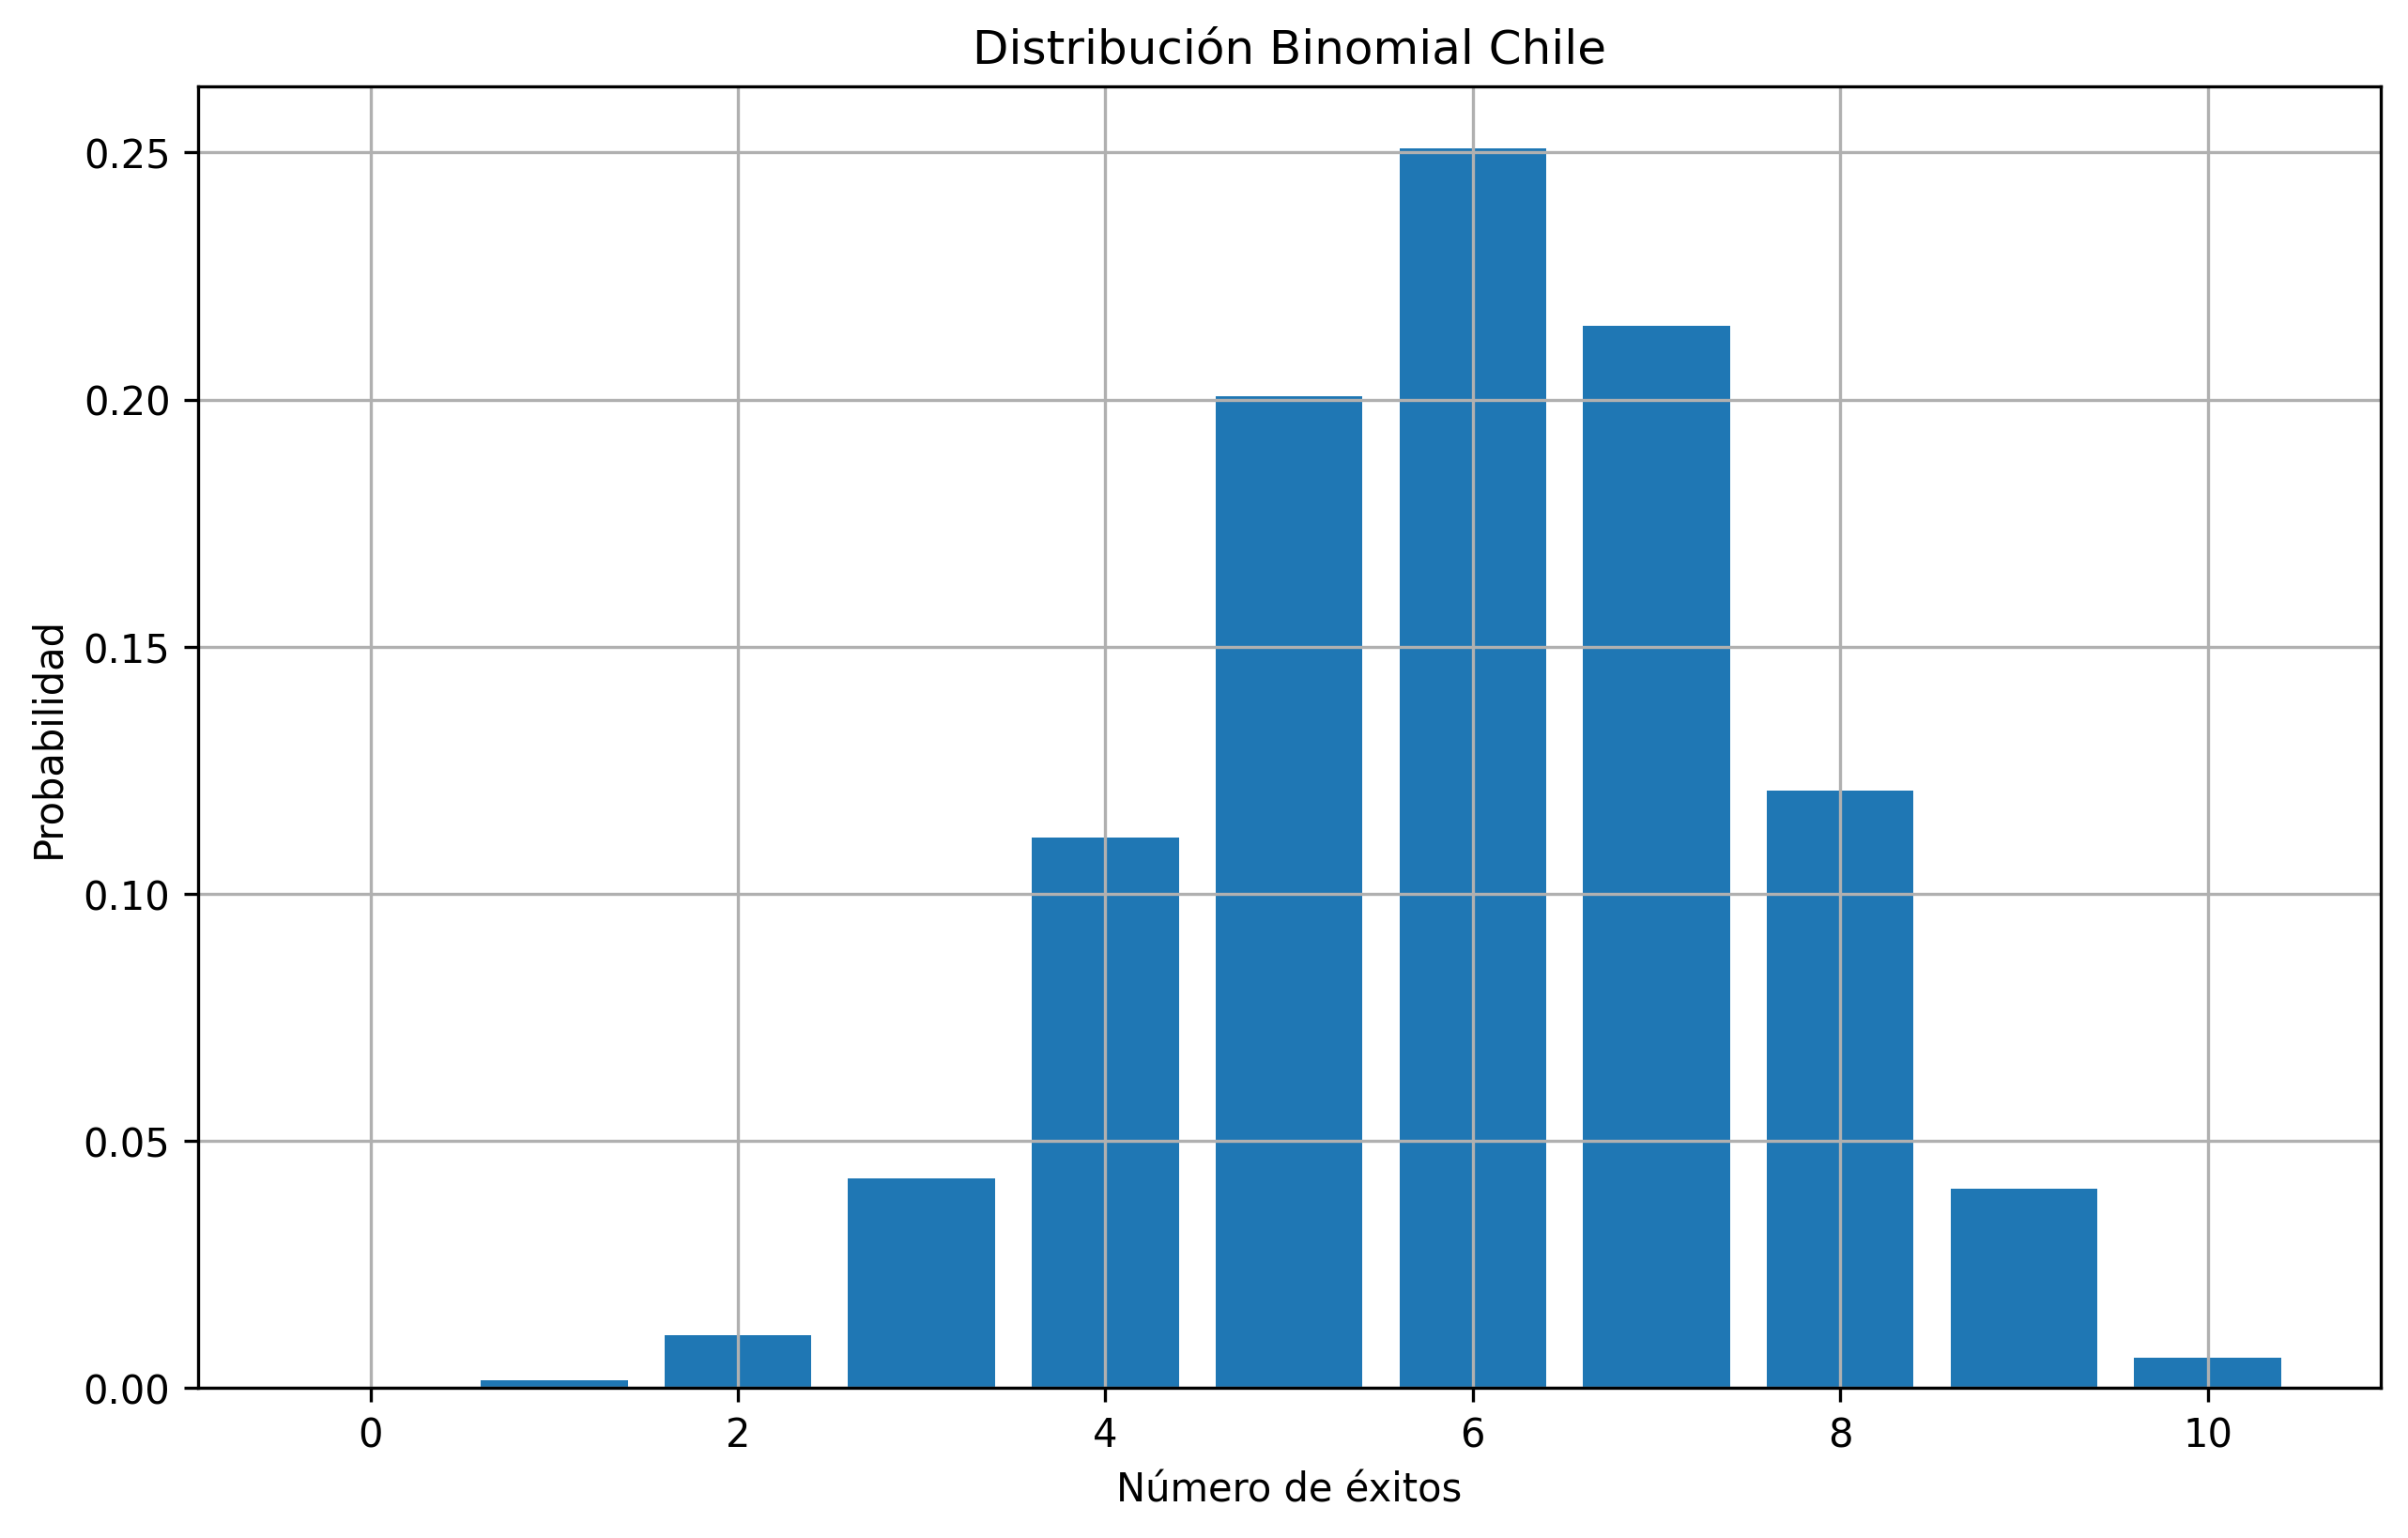
\includegraphics[width=0.8\textwidth]{grafica5.png}
\caption{Distribución Binomial}
\end{figure}

% =========================================================
% POISSON
% =========================================================

\subsection{Distribución Poisson}

\subsection*{Problema}

Calcular eventos económicos utilizando la distribución Poisson.

\subsection*{¿Por qué lambda = eventos/conteo?}

Porque representa el promedio de eventos por periodo.

\subsection*{Lambda}

\[
0.6
\]

\subsection*{Fórmula}

\[
P(x)=\frac{\lambda^x e^{-\lambda}}{x!}
\]

\subsection*{Resultado}

\[
3.55629940188929 \times 10^{-5}
\]

\subsection*{Interpretación}

La probabilidad de ocurrencia simultánea de varios eventos económicos es baja.

% =========================================================
% HIPERGEOMÉTRICA
% =========================================================

\subsection{Distribución Hipergeométrica}

\subsection*{Problema}

Calcular la probabilidad de seleccionar años con crecimiento económico sin reemplazo.

\subsection*{Fórmula}

\[
P(X=x)=
\frac{
\binom{K}{x}\binom{N-K}{n-x}
}{
\binom{N}{n}
}
\]

\subsection*{Resultado}

\[
0.47619047619047616
\]

\subsection*{Interpretación}

Existe una probabilidad moderada de seleccionar años con crecimiento económico dentro de la muestra.

% =========================================================
% NORMAL
% =========================================================

\subsection{Distribución Normal}

\subsection*{Problema}

Analizar los datos respecto a la media y desviación estándar.

\subsection*{Media}

\[
439391566.4297
\]

\subsection*{Desviación estándar}

\[
86707806.7008858
\]

\subsection*{Interpretación}

Los datos comerciales de Chile presentan una distribución cercana a una normal.

% =========================================================
% NORMAL ESTÁNDAR
% =========================================================

\subsection{Normal Estándar}

\subsection*{Problema}

Transformar los datos comerciales de Chile a puntuaciones Z.

\subsection*{Fórmula}

\[
Z=\frac{x-\bar{x}}{s}
\]

\subsection*{Resultados}

\[
-1.126419,\ -1.237429,\ -0.687032,\ -0.329595
\]

\subsection*{Interpretación}

Los valores negativos representan años por debajo del promedio y los positivos años por arriba del promedio.

% =========================================================
% INDICES
% =========================================================

\section{Índices Económicos}

% =========================================================
% PAASCHE
% =========================================================

\subsection{Índice Paasche}

\subsection*{Problema}

Comparar el comercio actual de Chile respecto al año base utilizando cantidades actuales.

\subsection*{Fórmula}

\[
P=\frac{\sum p_1 q_1}{\sum p_0 q_1}
\]

\subsection*{Resultado}

\[
1.6037935687972733
\]

\subsection*{Interpretación}

El comercio actual de Chile es mayor respecto al año base.

% =========================================================
% LASPEYRES
% =========================================================

\subsection{Índice Laspeyres}

\subsection*{Problema}

Comparar el comercio utilizando las cantidades del periodo base.

\subsection*{Fórmula}

\[
L=\frac{\sum p_1 q_0}{\sum p_0 q_0}
\]

\subsection*{Resultado}

\[
1.2858150890560203
\]

\subsection*{Interpretación}

El promedio comercial de Chile es superior respecto al periodo inicial.

% =========================================================
% FISHER
% =========================================================

\subsection{Índice Fisher}

\subsection*{Problema}

Calcular un índice equilibrado entre Paasche y Laspeyres.

\subsection*{Fórmula}

\[
IF=\sqrt{P\times L}
\]

\subsection*{Sustitución}

\[
IF=\sqrt{1.6037935687972733 \times 1.2858150890560203}
\]

\subsection*{Resultado}

\[
1.4360299337028244
\]

\subsection*{Interpretación}

El índice Fisher muestra un crecimiento comercial importante en Chile.

% =========================================================
% CONCLUSIÓN
% =========================================================

\section{Conclusión}

Con ayuda de datos reales obtenidos mediante la API oficial de OECD fue posible analizar el comportamiento comercial de Chile entre 2015 y 2024.

Los resultados muestran un crecimiento económico importante en los últimos años y permiten aplicar diferentes herramientas estadísticas para interpretar el comportamiento comercial del país.

Además, el uso de Python permitió automatizar cálculos, justificar fórmulas y generar gráficas que facilitan la comprensión de los resultados obtenidos.

\end{document}